\documentclass[11pt,a4paper]{article}

% --- Paquetes requeridos según especificación técnica ---
\usepackage[utf8]{inputenc}
\usepackage[T1]{fontenc}
\usepackage[spanish,es-nodecimaldot]{babel}
\usepackage[margin=2.5cm]{geometry}
\usepackage{graphicx}
\usepackage{booktabs}
\usepackage{tikz}
\usepackage{csquotes}
\usepackage[style=ieee,backend=biber]{biblatex}
\usepackage{hyperref}

% Configuración del archivo de bibliografía
\addbibresource{referencias.bib}

% Configuración de hipervínculos
\hypersetup{
    colorlinks=true,
    linkcolor=blue,
    filecolor=magenta,      
    urlcolor=cyan,
    citecolor=blue
}

\begin{document}

% ==============================================================================
% 1. CARÁTULA
% ==============================================================================
\pagenumbering{alph}
\begin{titlepage}
    \centering
    \vspace*{1cm}
    
    {\scshape\LARGE Universidad Técnica Estatal de Quevedo \par}
    \vspace{0.5cm}
    {\scshape\Large Facultad de Ciencias de la Ingeniería \par}
    \vspace{0.3cm}
    {\large Carrera de Ingeniería en Software / Computación \par}
    \vspace{1.5cm}
    
    {\huge\bfseries Informe Académico Individual: Análisis Crítico de un Sistema Distribuido Real \par}
    \vspace{0.5cm}
    {\Large\bfseries MinIO frente a Apache HDFS \par}
    \vspace{0.5cm}
    {\large Actividad: TA-IND-01 (Semana 3) \par}
    \vspace{2cm}
    
    \begin{flushleft}
        \textbf{Asignatura:} Sistemas Distribuidos \\
        \textbf{Estudiante:} Heiner Ariel Zambrano Ronquillo \\
        \textbf{Paralelo:} % TODO: Indicar paralelo (ej. 7mo "A")
        \\
        \textbf{Fecha de Entrega:} 13 de noviembre de 2026 \\
        \textbf{Repositorio GitHub:} % TODO: Colocar URL completa del repositorio (en una sola línea)
    \end{flushleft}
    
    \vfill
    {\large Quevedo -- Ecuador \par}
    {\large 2026 \par}
\end{titlepage}

\newpage
\pagenumbering{roman}
\tableofcontents
\newpage
\pagenumbering{arabic}

% ==============================================================================
% 2. RESUMEN
% ==============================================================================
\section{Resumen}
\newpage

% ==============================================================================
% 3. INTRODUCCIÓN
% ==============================================================================
\section{Introducción}

% ==============================================================================
% 4. ARQUITECTURA DEL SISTEMA
% ==============================================================================
\section{Arquitectura del Sistema}

% ==============================================================================
% 5. ANÁLISIS CON LOS CONCEPTOS DE LA UNIDAD 1
% ==============================================================================
\section{Análisis con los Conceptos de la Unidad 1}

\subsection{Transparencias de Distribución}

\subsection{Teorema CAP y PACELC}

\subsection{Modelos de Comunicación}

\subsection{Tolerancia a Fallos}

% ==============================================================================
% 6. EXPERIMENTACIÓN PROPIA
% ==============================================================================
\section{Experimentación Propia}

% ==============================================================================
% 7. EJEMPLOS DEL ENTORNO DEL ESTUDIANTE
% ==============================================================================
\section{Ejemplos del Entorno del Estudiante}

% ==============================================================================
% 8. ANÁLISIS COMPARATIVO
% ==============================================================================
\section{Análisis Comparativo: MinIO frente a Apache HDFS}

% ==============================================================================
% 9. POSTURA CRÍTICA
% ==============================================================================
\section{Postura Crítica}

% ==============================================================================
% 10. CONCLUSIONES
% ==============================================================================
\section{Conclusiones}
\section{Declaración de Uso de Inteligencia Artificial}
\newpage
\printbibliography[heading=bibintoc,title={Referencias}]
\newpage
\appendix
\section{Anexo A: Esquema Inicial de Arquitectura a Mano Alzada}
% Evidencia obligatoria de autoría (D3): fotografía del bosquejo inicial dibujado a mano por el estudiante.
\begin{figure}[htbp]
    \centering
    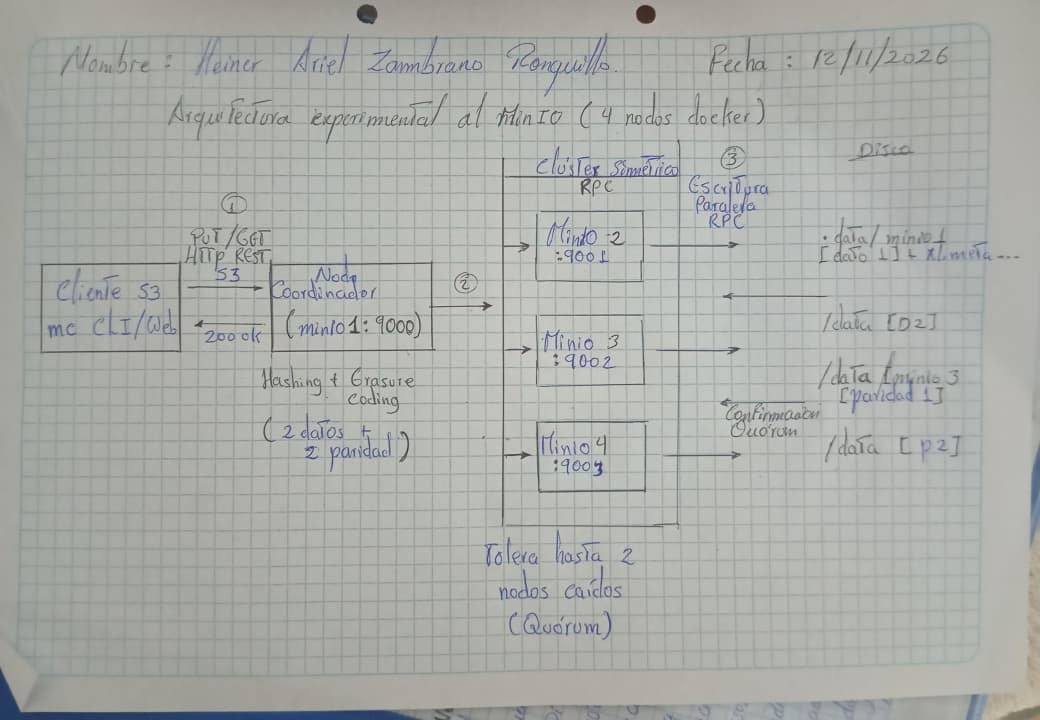
\includegraphics[width=0.92\textwidth]{../figura/bosquejo_inicial_amano.jpeg}
    \caption{Bosquejo inicial a mano alzada de la arquitectura experimental de MinIO distribuido (Anexo A).}
    \label{fig:anexo_a_bosquejo}
\end{figure}

\section{Anexo B: Evidencia de Lectura Crítica de Fuentes Bibliográficas}
\end{document}
